\documentclass[varwidth=true, border=2pt]{standalone}

\usepackage{pgfplots}
\usepackage{tikz}

\begin{document}
	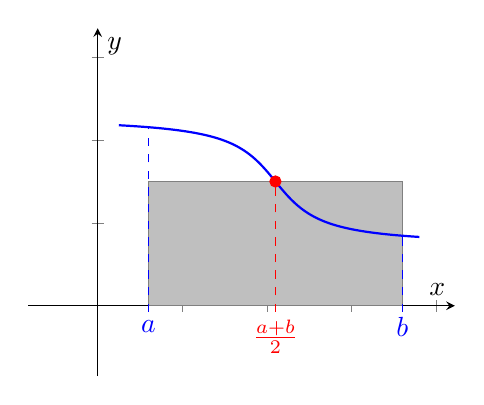
\begin{tikzpicture}
    \begin{axis}[
        legend pos=south east,
        axis x line=middle,
        axis y line=middle,
	xticklabels=\empty,
	yticklabels= \empty,
        grid = none ,
        width=7cm,
        height=6cm,
        grid style={dashed, gray!1},
        xmin=-2,     % start the diagram at this x-coordinate
        xmax=19,    % end   the diagram at this x-coordinate
        ymin=-1,     % start the diagram at this y-coordinate
        ymax= 6,   % end   the diagram at this y-coordinate
        xlabel=$x$,
        ylabel=$y$,
        enlargelimits=true,
        tension=0.08]

\filldraw[fill=lightgray, draw=gray] (axis cs: 3,0) rectangle (axis cs: 18,3);


 \addplot[domain=1.25:19, blue, thick,samples=250] {rad(-atan(x/2-5.25))+3}; % Parabola
  \addplot[red, only marks, mark=*] coordinates {(10.5,3)};
  \draw [blue,dashed] (axis cs: 3,-0.15) -- (axis cs: 3,4.31);
     \draw [red,dashed] (axis cs: 10.5,-0.15) -- (axis cs: 10.5,3);
  \draw [blue,dashed] (axis cs: 18,-0.15) -- (axis cs: 18,1.68);
  

	\node(a)[blue] at (axis cs: 3,-0.5){$a$};
	\node(b)[blue] at (axis cs: 18,-0.5){$b$};
	\node(MP)[red] at (axis cs: 10.5,-0.75){$\frac{a+b}{2}$};
    \end{axis}
\end{tikzpicture}
\end{document}